% Complex points z_i (red) and their upper-half square roots w_i (blue).
% Faithful redraw of the Asymptote diagram in book/tex/complex-ana/log.tex.
\documentclass[border=2mm]{standalone}
\usepackage{tikz}\usetikzlibrary{arrows.meta}
\begin{document}
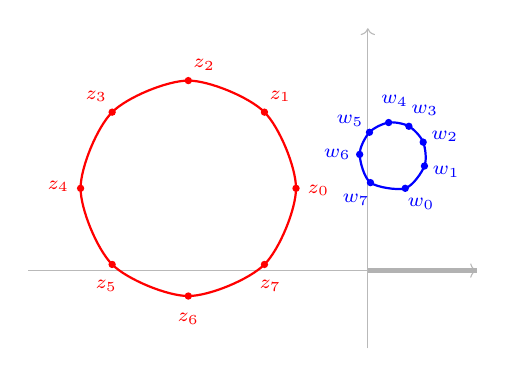
\begin{tikzpicture}[scale=0.95]
  \draw[->,gray!55] (-4.54,0) -- (1.46,0);
  \draw[->,gray!55] (0,-1.04) -- (0,3.24);
  \draw[gray!60,line width=1.6pt] (0,0) -- (1.46,0);
  \draw[red,thick] plot[smooth cycle] coordinates {(-0.960,1.100) (-1.382,2.118) (-2.400,2.540) (-3.418,2.118) (-3.840,1.100) (-3.418,0.082) (-2.400,-0.340) (-1.382,0.082)};
  \fill[red] (-0.960,1.100) circle (1.4pt); \node[red,font=\scriptsize] at (-0.661,1.074) {$z_{0}$};
  \fill[red] (-1.382,2.118) circle (1.4pt); \node[red,font=\scriptsize] at (-1.170,2.330) {$z_{1}$};
  \fill[red] (-2.400,2.540) circle (1.4pt); \node[red,font=\scriptsize] at (-2.188,2.752) {$z_{2}$};
  \fill[red] (-3.418,2.118) circle (1.4pt); \node[red,font=\scriptsize] at (-3.630,2.330) {$z_{3}$};
  \fill[red] (-3.840,1.100) circle (1.4pt); \node[red,font=\scriptsize] at (-4.139,1.126) {$z_{4}$};
  \fill[red] (-3.418,0.082) circle (1.4pt); \node[red,font=\scriptsize] at (-3.496,-0.208) {$z_{5}$};
  \fill[red] (-2.400,-0.340) circle (1.4pt); \node[red,font=\scriptsize] at (-2.400,-0.640) {$z_{6}$};
  \fill[red] (-1.382,0.082) circle (1.4pt); \node[red,font=\scriptsize] at (-1.304,-0.208) {$z_{7}$};
  \draw[blue,thick] plot[smooth cycle] coordinates {(0.500,1.100) (0.757,1.398) (0.740,1.717) (0.549,1.929) (0.278,1.979) (0.022,1.849) (-0.109,1.553) (0.035,1.176)};
  \fill[blue] (0.500,1.100) circle (1.4pt); \node[blue,font=\scriptsize] at (0.712,0.888) {$w_{0}$};
  \fill[blue] (0.757,1.398) circle (1.4pt); \node[blue,font=\scriptsize] at (1.047,1.321) {$w_{1}$};
  \fill[blue] (0.740,1.717) circle (1.4pt); \node[blue,font=\scriptsize] at (1.030,1.794) {$w_{2}$};
  \fill[blue] (0.549,1.929) circle (1.4pt); \node[blue,font=\scriptsize] at (0.761,2.141) {$w_{3}$};
  \fill[blue] (0.278,1.979) circle (1.4pt); \node[blue,font=\scriptsize] at (0.356,2.269) {$w_{4}$};
  \fill[blue] (0.022,1.849) circle (1.4pt); \node[blue,font=\scriptsize] at (-0.238,1.999) {$w_{5}$};
  \fill[blue] (-0.109,1.553) circle (1.4pt); \node[blue,font=\scriptsize] at (-0.409,1.553) {$w_{6}$};
  \fill[blue] (0.035,1.176) circle (1.4pt); \node[blue,font=\scriptsize] at (-0.158,0.946) {$w_{7}$};
\end{tikzpicture}\end{document}
